\documentclass[draft,jgrga]{agutex}

%  Uncomment the following command to include .eps files
\usepackage{graphicx}
%
%  Uncomment the following command to allow illustrations to print
%   when using Draft:
\setkeys{Gin}{draft=false}

% Author names in capital letters:
\authorrunninghead{HINES AND HETLAND}

% Shorter version of title entered in capital letters:
\titlerunninghead{RHEOLOGIC CONSTRAINTS ON THE MANTLE}

%Corresponding author mailing address and e-mail address:
\authoraddr{Corresponding author: T. T. Hines,
Department of Earth and Environmental Sciences, University of
Michigan, 2534 C. C. Little Building, 1100 North University Avenue,
Ann Arbor, MI 48109-1005. (hinest@umich.edu)} 

\begin{document}

\title{Supporting Information for ``Rheologic constraints on the upper mantle from five years of postseismic deformation following the El Mayor-Cucapah earthquake"}

\authors{Trever T. Hines,\altaffilmark{1}
         Eric A. Hetland,\altaffilmark{1}}

\altaffiltext{1}{Department of Earth and Environmental Sciences, University of Michigan, Ann Arbor, Michigan, USA.}

\begin{article}

\noindent\textbf{Contents of this file}

\begin{enumerate}
\item Figures S1 to S4
\end{enumerate}
\noindent\textbf{Introduction}

Figures S1 and S2 provide additional information about the inversion in Section 3.2 of the main text. Figures S3 and S4 show the predicted displacements, which have been decomposed into elastic and viscoelastic components, for the preferred model from Section 3.3.  
  
\end{article}
\clearpage

\begin{figure}
\setfigurenum{S1} %%Change number for each figure
\noindent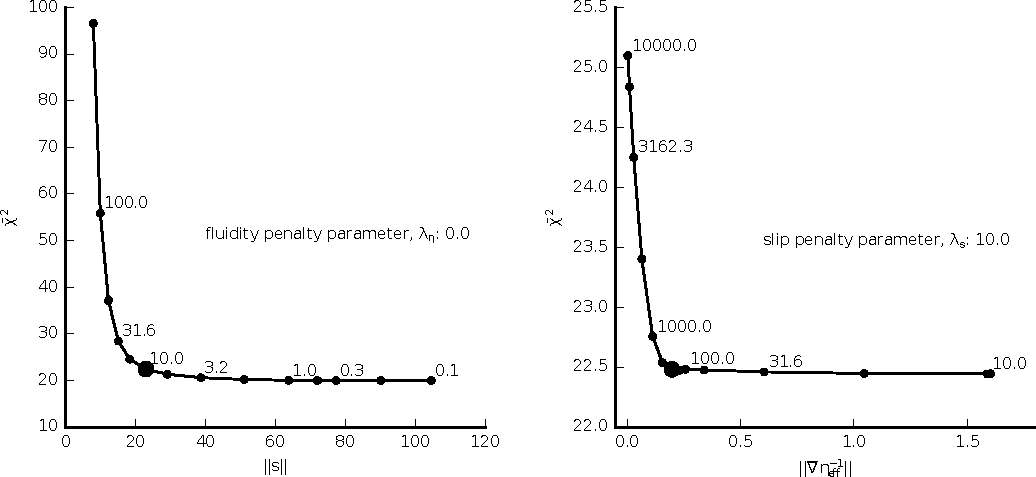
\includegraphics[scale=1.0]{Figures/2016jb013114-fS01}
\caption{
Trade-off curves used to determine the damping parameters $\lambda_s$ and $\lambda_\eta$ in eq. (15) of the main text.  The left panel shows the trade-off curve for the fault slip penalty parameter, $\lambda_s$.  We pick $\lambda_s$ while keeping the penalty parameter for fluidity, $\lambda_\eta$, fixed at zero.  The right panel shows the trade of curve for selecting $\lambda_\eta$, where we fix $\lambda_s$ at the chosen value from the left panel. Chosen values are indicated with the larger marker.  When picking $\lambda_s$, we try to find a good balance between the mean chi-squared value, $\bar{\chi}^2$, and the size of the slip parameters, $||s||$.  Our choice of $\lambda_\eta$ is a balance between $\bar{\chi}^2$ and the size of the Laplacian of fluidity, $||\nabla \eta_\mathrm{eff}^{-1}||$. 
}
\label{fig:S1}
\end{figure}

\begin{figure}
\setfigurenum{S2} %%Change number for each figure
\noindent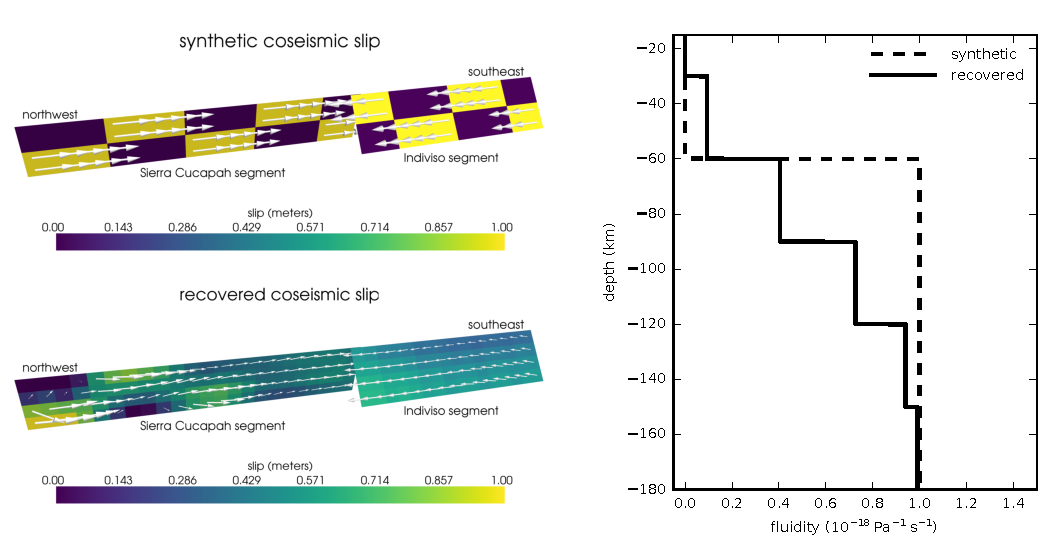
\includegraphics[scale=1.0]{Figures/2016jb013114-pS02}
\caption{
Checkerboard test used to assess the resolving power of the inversion in Section 3.2 of the main text.  We create synthetic data at all of the GPS stations considered in this study by evaluating eq. (14) with the synthetic coseismic slip distribution and fluidity distributions. Our synthetic fluidity model has a jump from 0.0 to $10^{-18}$ Pa$^{-1}$ s$^{-1}$ at 60 km depth.  Our synthetic slip model does not include afterslip, although we estimate afterslip along with coseismic slip and fluidity in this test.  We estimate these values in the same way as described in the main text and we also use the same penalty parameters.  We do not add any noise to our synthetic data so that the recovered model just indicates how much the regularization influences the solution.  Note that our ability to recover slip decreases towards the southern end of the fault, farthest from the available data.  Also note that the smoothing constraint on fluidity largely obscures the jump in the synthetic model.
}
\label{fig:S2}
\end{figure}

\begin{figure}
\setfigurenum{S3} %%Change number for each figure
\noindent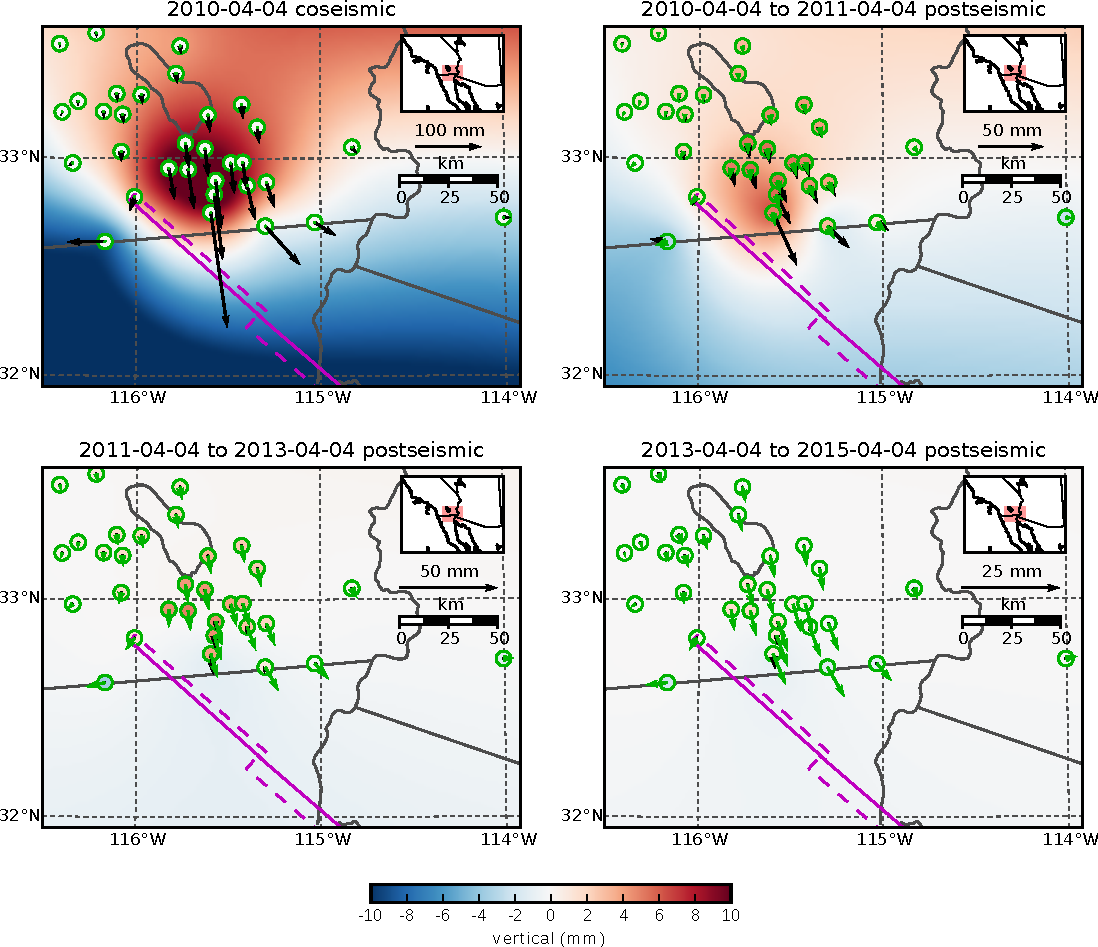
\includegraphics[scale=0.9]{Figures/2016jb013114-pS03}
\caption{
Elastic (black) and viscoelastic (green) components of the near-field predicted displacements for the preferred Zener model from Section 3.3.  The elastic component is the deformation resulting from fault slip and the viscoelastic component is the deformation resulting from viscoelastic relaxation of stresses induced by the fault slip.  The elastic and viscoelastic components are calculated from the first and second terms in eq. (11), respectively.  The vertical elastic component is shown as an interpolated field and the vertical viscoelastic component is shown within the green circles.  
}
\label{fig:S3}
\end{figure}

\begin{figure}
\setfigurenum{S4} %%Change number for each figure
\noindent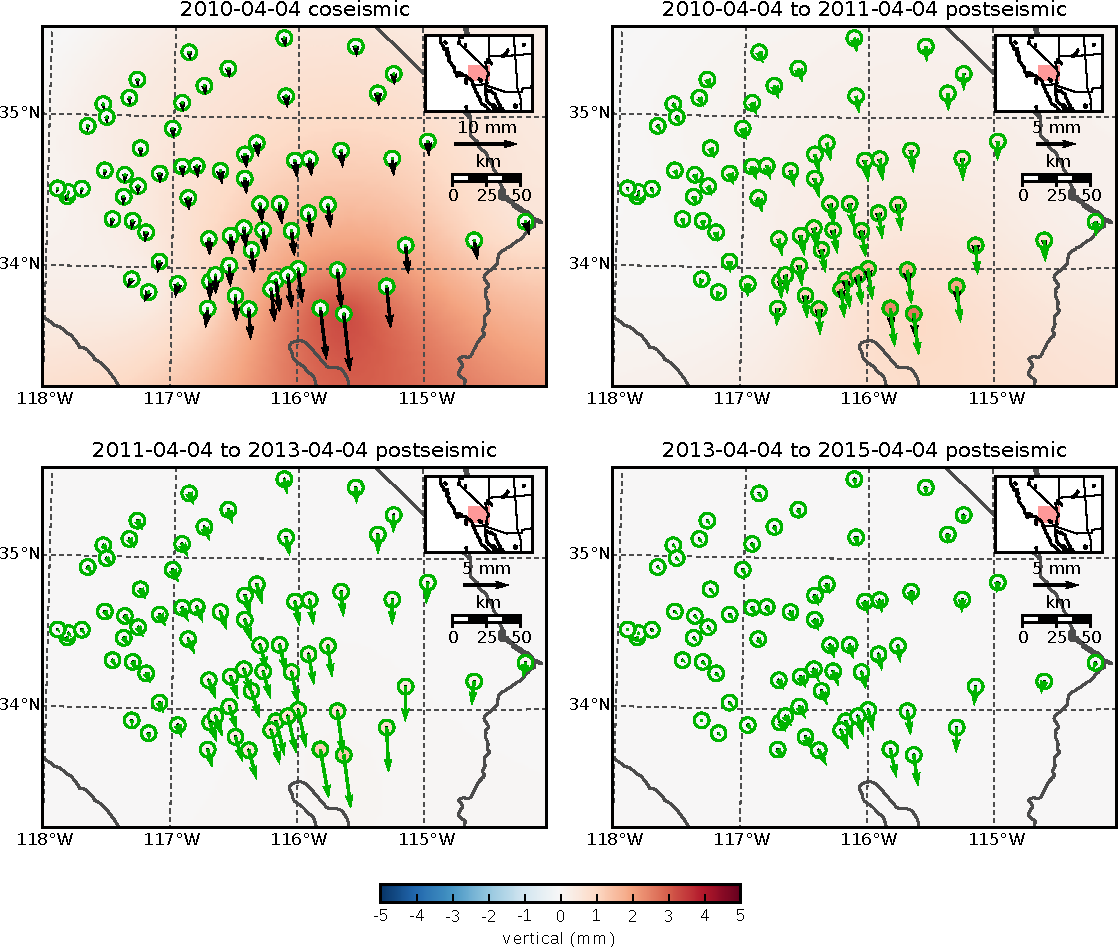
\includegraphics[scale=0.9]{Figures/2016jb013114-pS04}
\caption{
Same as figure S3 but for far-field stations.
}
\label{fig:S4}
\end{figure}

\end{document}

